\section{OpenCL}

\subsection{Language Overview}

Open Computing Language (OpenCL) is a framework for writing applications
designed to be executed across heterogeneous platforms such as central
processing units (CPUs), graphics processing units (GPUs), and accelerator
devices such as the Intel Phi and Field Programmable Gate Arrays (FPGAs). The
language is an open standard maintained by Khronos Group
\footnote{\url{http://www.khronos.org/opencl}}. OpenCL is based on the C99
standard and can be loosely thought of as a subset of the C99 language with some
additional keywords. The first release of the OpenCL standard (OpenCL 1.0) was
on the 8th of December 2008. There have been two subsequent stable releases of
the standard, OpenCL 1.1 and 1.2, on the 14th of June 2010 and 15th of November
2011 respectively. The version with most hardware support is OpenCL 1.1
\footnote{\url{http://www.khronos.org/registry/cl/specs/opencl-1.1.pdf}} and
this standard forms the basis of all discussion on OpenCL in this report.

OpenCL splits the program code into two sections called `host' and `device'.
Host code runs on the CPU and is written in a traditional language such as C or
C++. The host code executes as normal and makes use of APIs exposed by OpenCL to
define how, and where, OpenCL device code is executed.

OpenCL applications are called kernels. A kernel is a function that executes on
an OpenCL capable device. Given the focus of OpenCL is on parallelism, a kernel
is written from the perspective of a single thread instead of requiring explicit
threading code from more familiar models such as POSIX Threads. An OpenCL work
item is similar to a POSIX Thread with a notable exception that OpenCL has no
traditional stack, any `function' calls are actually in-lined by the compiler.
OpenCL kernels are also compiled at runtime thus the host code, and the compiler
itself, can make device-specific optimisations for optimal performance.

\subsection{Models}

To accommodate the variety of devices OpenCL is designed to work with, a more
abstract Memory Model, and Concurrency and Execution model was designed to allow
the programmer full access to the target devices' capabilities.

\subsubsection{Memory Model}

For a traditional C/C++ application, the application programmer can make use of
the primary memory space of the computer, typically DDR2 or DDR3 RAM. There are
caches on the CPU die however no direct control over their contents is offered.
For CPUs this is not an issue, all modern CPUs support automatic caching.
Problems occur when considering other devices, such as a GPU. GPUs do not
typically have automatic caching thus a programmer must make use of OpenCLs
abstract memory model, and hardware vendors must map this model to the physical
hardware. The OpenCL memory model defines four different types of memory, each
of which will be outlined below. A simplified diagrammatic representation of the
memory model is shown in Figure \ref{fig:openCLMemoryModel}.

\begin{description}

\item[Global memory] This memory is accessible by all compute units and is
similar to main memory on a traditional CPU system. All work items are able to
access and update everything stored in this memory. For a GPU this is memory is
mapped to the primary memory of the GPU and is typically 1-4GB in size. When
transferring data between the host and device, this is where the data has to
reside. Global memory is denoted as `\_\_global' in an OpenCL kernel.

\item[Constant memory] Constant memory resides in the same space as global
memory and is used for data which is accessed simultaneously by all work items,
or for variables whose values never change. Constant memory is denoted as
`\_\_constant' in an OpenCL kernel.

\item[Local memory] This is scratch pad memory which is only visible to a single
compute unit on the device. Local memory can be split up into distinct sections
if a single compute unit is executing multiple work- groups simultaneously.
Local memory is generally on- chip memory and thus has faster access time than
global memory. Local memory is typically on the order of tens of kilobytes in
size. Use of local memory is either statically declared in the kernel (e.g
`\_\_local float[64] localArray') or dynamically allocated at runtime by the
host since OpenCL kernels do not offer dynamic memory allocation. Variables in
local memory are not what would be called `local' in a traditional application,
local variables are in private memory. Variables in local memory are shared
across a single work group, which can contain multiple work items.

\item[Private memory] This is memory that is unique to an individual work item.
Any local variables and non-pointer kernel arguments are private by default.
These are typically mapped to registers although thy can be spilled over to
higher latency memories if there is insufficient space available.

\end{description}

\begin{figure}
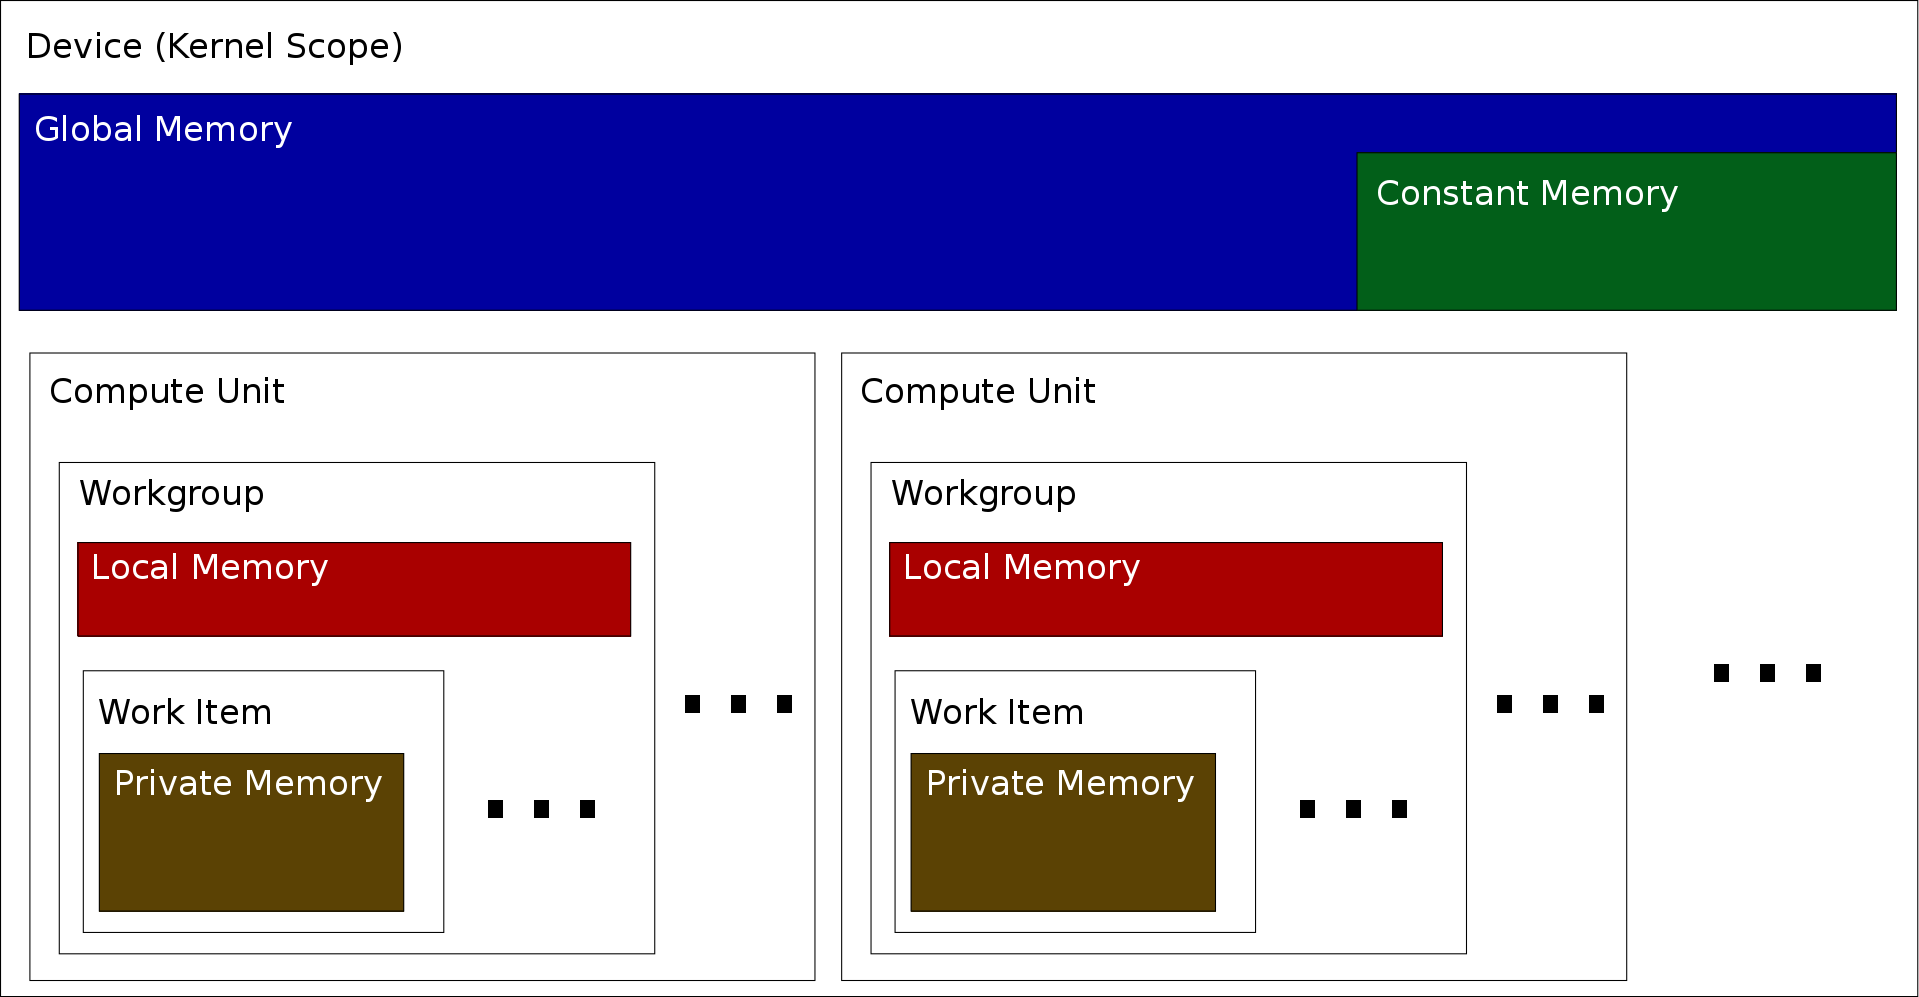
\includegraphics[width=\linewidth]{images/openCLMemoryModel.png}
\caption{Simplified visualisation of OpenCL Memory Model}
\label{fig:openCLMemoryModel}
\end{figure}

\subsubsection{Concurrency and Execution Model}

As shown in Figure \ref{fig:openCLMemoryModel}, OpenCL uses a number of
different terms to describe it's execution model. There is no explicit `thread',
instead OpenCL has work items which are the closest relative to traditional
threads. The OpenCL Concurrency and Execution Model is split into two parts,
host and device, and both will be outlined below.

\paragraph{Host}

\begin{description}

\item[Host program] As discussed previously, a host program is a traditional
program (written in C/C++ for instance) and is executed on a CPU. The host
program is responsible for managing the execution of kernels by creating and
setting up command queues for memory commands, kernel execution commands, and
synchronisation of commands.

\item[Context] The host program defines a context for the kernels. The context
will include the kernels to be executed, the available OpenCL devices, the
program kernels, and the memory objects used by kernels.

\item[NDRange] This stands for N-Dimensional Range and defines how work items
are organised. Work items can be arranged into 1, 2, or 3 dimensions. This can
be done to increase performance and improve clarity of kernel code. For
instance, modifying an image would warrant having a two dimensional range as an
image is represented as a two dimensional array of pixels.

\item[Device Type] OpenCL places devices into three different classifications.
CPUs, GPUs, and Accelerators. An example accelerator device would be the Intel
Phi \footnote{\url{http://www.intel.com/content/www/us/en/processors/xeon/xeon-
phi-detail.html}}.

\end{description}

\paragraph{Device}

\begin{description}

\item[Compute Unit] This is a generic term used to describe a multiprocessor on
a GPU, or a core of a CPU. For some devices (such as a GPU) a compute unit will
have dedicated local memory, visible only to itself. A single compute unit can
be assigned multiple work groups.

\item[Kernel] As discussed previously, OpenCL code which runs on an OpenCL
device is known as a kernel. These are written from the perspective of a single
work item (thread).

\item[Work group] This is a collection of work items. An entire work group is
assigned to one compute unit. These work items can share local memory and can
synchronise with one another.

\item[Work item] This closely resembles a single thread. Each work item is
assigned a work group. Every work item can access local memory of its work
group and can access all global and constant memory. A work item will also
have private variables which may or may not fit inside private memory.

\item[Global size] This represents the total number of work items in each
dimension. The multiplication of the global size in each dimension is the total
number of work items being executed for the corresponding kernel.

\item[Local size] This represents the total number of work items in each
dimension for a single work group. The global size for a dimension has to be an
integer multiple of the local size for that dimension for the work group size
to be valid. This is to ensure work groups can fit inside the global dimension
size evenly.

\end{description}

Just as with the Memory Model, different devices will realise the Concurrency
and Execution model differently. These differences will be discussed in the next
section.

\section{Device comparisons}

There are numerous important architecture differences between different classes
of device. At the high level, CPUs are aimed at being good all-rounders,
suitable for a multitude of tasks whereas GPUs have focused on the problem of
pixel value generation in a highly parallel fashion. This had led to the
evolution of different devices taking distinct paths. The important differences
will be outlined in this section.

\subsection{CPU and GPU}

The CPU is typically referred informally as the `brain' of the computer, not
only does it run the user's wide variety of software, it also acts as the
overall controller for the entire system. This necessitated a one-size-fits-all
style of approach when designing the CPU chip and the corresponding instruction
set architecture. A CPU typically has a high clock speed, in the range of 3-4GHz
for a modern desktop. Each die can contain a small number, typically four, of
cores that execute instructions independently.

A GPU is the highly parallel oriented chip, with hundreds of cores running at a
slower clock speed (about one fifth of a CPU core) and have a more restricted
instruction set, primarily designed for simple, repetitive tasks needed for
video output.

\subsubsection{Threading and Cache}

A CPU has a few hardware threads, 1 or 2 per CPU core, and multi-level cache to
reduce off-chip memory access latency.

GPUs have many threads to keep compute units busy, if some threads are waiting
on memory accesses, other threads are available to run. Latency is thus hidden
rather than reduced. This has led to the context switch cost for GPU threads to
be insignificant.

\subsubsection{Arithmetic Throughput}

GPUs use more of the transistor budget on arithmetic units than memory cache
compared to CPUs. This lends GPUs to high density arithmetic and repetitive
computations more than a CPU.

\subsubsection{Execution Model Implementation}

CPUs have a very free implementation of the OpenCL execution model. Threads are
free to take their own execution path, and aren't directly affected by other
thread's progress except from at explicit synchronisation stages.

GPUs, on the other hand, have a Single Instruction Multiple Threads (SIMT)
execution model. This means that GPUs have one instruction unit for multiple
arithmetic units. Threads are partitioned into groups which execute the same
instruction simultaneously. For nVidia GPUs these are referred to in the CUDA
model as `warps' and typically contain 32 threads. This can increase performance
as this reduces the number of fetch and decode operations on instructions
required. A performance consequence of this is in code with conditional
branches.

\begin{verbatim}
if (someCondition)
{
    nonTrivialCode();
}
else
{
    someMoreNonTrivialCode();
}
\end{verbatim}

For a simple example, consider the situation when someCondition is true for half
of the threads, and false for the other half threads. For a CPU each thread
executes the instructions by itself and some threads can be executing
`nonTrivialCode()' at the same time some threads are executing
`someMoreNonTrivalCode()'. However, on a GPU the threads in the true branch
execute their instructions while the other threads remain idle, after the true
branch has been completed, the false branch threads then execute, this is known
as a divergent warp. Divergent warps can considerably reduce performance as it
reduces the number of threads executing in parallel.

In addition to instruction execution, memory accesses are done on a per warp
basis. For ideal performance addressing should be such that threads in a warp
access coalesced memory locations to reduce memory transaction cost. For
instance, an array where access is based on a hash function can result in poor
performance as threads in a warp are likely to be accessing significantly
different parts of memory.

\subsubsection{Extra performance consideration}

In addition to the architecture differences between CPUs and GPUs, there is a
separate consideration that must be made for GPUs and other discrete devices,
the PCI-E bus. GPUs are unable to directly access main memory like a CPU, thus
before any code is run on a GPU, data must be transferred between RAM and the
GPUs on-board memory. This can take a significant period of time in comparison
to the code runtime. This is due to the relatively slow speed of the PCI-E bus
in comparison to on-board memory access. A GPU is able to access it's global
memory at a rate of around 200GB/s on modern chips. Contrast this to the PCI-E
link speed which can be as low as 250MB/s per lane. The most common systems have
PCI-E 2.0 slots which run at 500MB/s per PCI-E lane with 16 lanes available for
the GPU giving a maximum theoretical transfer speed of 8GB/s, 25 times slower
than access from on-board memory.

\subsection{Bridging the gap - APUs}

Both CPUs and GPUs are strong in their respective application areas. Ideally, a
system should be able to make best use of both types of device with as little
overhead as possible. One of the obvious potential bottlenecks is the PCI-E bus
to devices discrete from the CPU. This led to the design of an Accelerated
Processing Unit (APU), these have a traditional CPU in addition to a GPU (or
FPGA) on the same die and are a good example of a Heterogeneous System
Architecture (HSA). This design isn't new, CPUs have typically contained a small
GPU, especially in the small laptop market. With the growth of Heterogeneous
Systems, there has been a trend to increasing the GPU performance on die with
the CPU. This reduces the gap between CPU and GPU and removes the PCI-E bus
overhead. The primary consumer implementation of this is AMDs HSA
\footnote{\url{http://developer.amd.com/resources/heterogeneous-computing/}}.
The joint die allows power to be managed so that different applications can make
most effective use of the CPU and GPU cycles available. In addition, there is
also work going on to completely unify address space, to make the heterogeneous
architecture more seamless to work with.

For the purposes of this report, APU discussion ends here. At present consumer
devices are relatively immature and for a majority of applications, a distinct
GPU or accelerator card is more likely to achieve the best overall performance.

\subsection{Intel Phi}

\section{Document Classification}

\subsection{Bloom Filters}

\subsection{Hashed Profile}

% linear probing, hence 4 terms looked at.
